\section{Introducción}
Los filtros pasabajas, son un tipo de filtro los cuales permiten que las frecuencias menores a una frecuencia de corte (fc) ``pasen'' normalmente y las posteriores a esta son filtradas (es decir, no aparecen en la salida). Teóricamente, estos filtros deben de rechazar las frecuencias mayores a la frecuencia de corte, pero en la práctica, estos filtros atenúan las frecuencias mayores a la frecuencia de corte a cierta velocidad de decaimiento según sea el orden del filtro (1er orden-20dB/década, 2do orden-40dB/década, etc). Los filtros ideales no son posibles de implementar, pero existen diversas implementaciones de filtros que buscan acercase lo más posible a un filtro ideal.\\ La implementación más sencilla de un filtro pasabajas es la obtenida con un circuito RC (Resistencia-Capacitor), el cual es representado en la Figura 1.
\begin{figure}[H]
	\centering
	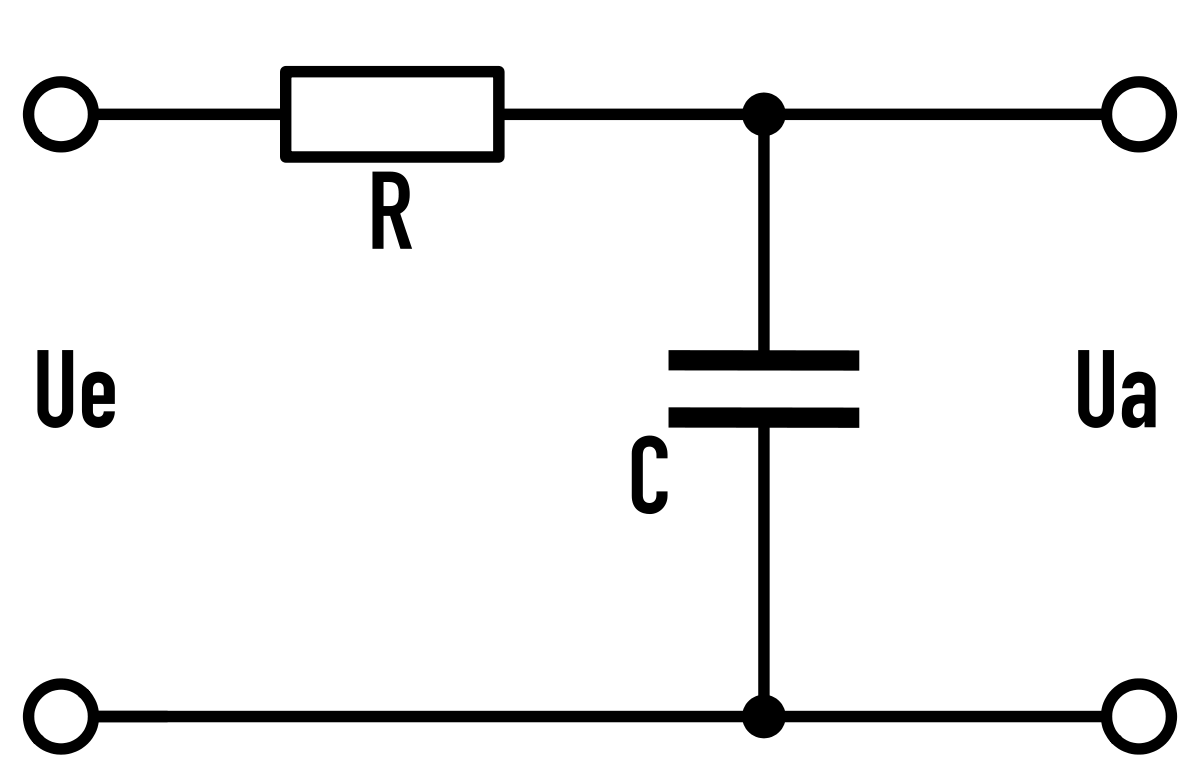
\includegraphics[scale=.14]{img/rc.png}
	\caption{Circuito RC}
	\label{fig:CircuitoRC}		
\end{figure}
La forma del filtro pasabajas en frecuencia, se puede observar en la Figura 2.
\begin{figure}[H]
	\centering
	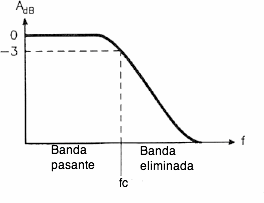
\includegraphics[scale=.9]{img/filtro.png}
	\caption{Diagrama de Bode para un filtro pasabajas}
	\label{fig:FrecuenciaRC}		
\end{figure}
Donde la frecuencia de corte esta dada por:
\begin{center}
	$ {w}_{c}=\frac{1}{RC}$ \\ $ {w}_{c}=2\pi {f}_{c}$
\end{center}
Como se puede observar, la frecuencia de corte depende enteramente de la resistencia y capacitor, a esta clase de filtros también se le conoce como pasivos, ya que están compuestos puramente por elementos de este tipo.\\ Al analizar el circuito, se obtiene que la función de transferencia del mismo es:
\begin{center}
	$ {H}_{\left(s \right)}=\frac{1}{1+RsC} $
\end{center}
Donde s, es un número complejo; s=jw.\\
De la anterior función de transferencia, podemos obtener la respuesta al impulso del circuito (la inversa de la transformada de Laplace de la función de transferencia), esto representa la respuesta del circuito a una entrada de voltaje consistente en un impulso o función delta de Dirac.
\begin{center}
	$ \frac{1}{RC}{e}^{-\frac{1}{RC}t}u \left(t\right) $
\end{center}
Si se sustituye ${w}_{c}=\frac{1}{RC}$ se obtiene lo siguiente:
\begin{center}
	$ {w}_{c}{e}^{-{w}_{c}t}u \left(t\right) $
\end{center}
De tal manera, es posible modelar el filtro sin necesidad de proponer un valor para la resistencia y el capacitor, tan solo es necesario conocer la frecuencia de corte deseada. Esto resulta útil al momento de realizar un programa que simule este tipo de filtro. Esta simulación, se puede obtener mediante la convolución de dos señales (la señal de entrada y la respuesta al impulso del circuito RC).\\ \textbf{La convolución} es un operador matemático que transforma dos funciones f y g en una tercera función que representa la magnitud en la que se superponen f y una versión trasladada e invertida de g. 